% Project Specifications

\chapter{The Generator Model}

In this chapter, a brief description of \gls{gan} \cite{goodfellow:gan} is presented first, followed by the
structure of the generator in the \gls{dcgan} model used in this project. There are three types of layers in
the model: a transposed convolutional layer that performs upscaling to its input, a batch normalization layer
that improves model stability and accuracy, an activation layer that introduces nonlinearity to the model.
The main focus is on the transposed convolutional layer, which is the core of the generator model.

\section{A Description of \gls{gan}}

There are two networks in a \gls{gan} model: $D$, the discriminator, and $G$, the generator. $D$ is a
discriminative model which computes a function $D: \boldsymbol{x} \rightarrow p$ where $\boldsymbol{x}$ is the
input example and $p \in \mathbb{R}$ is the probability that $\boldsymbol{x}$ came from real training data
rather than data generated by $G$. In a sense, this probability value identifies the input example as
``authentic'' or not, so the higher the probability, the better $D$ does at discriminating authentic data
against data ``faked'' by $G$. On the other hand, $G$ tries to fool $D$ by generating output that resembles
the real data, and learns the data distribution during the training process. The input to $G$ is a vector
$\boldsymbol{z}$ of random noises which could be drawn from a normal distribution, so $G: \boldsymbol{z}
\rightarrow \boldsymbol{x}$ is a mapping from the $\boldsymbol{z}$ space to the data space $\boldsymbol{x}$.

During the training, two types of examples are fed to $D$: existing training examples and examples generated
by $G$. The system can be trained with regular \gls{sgd} and backpropagation. The training
process improves the ability of both $D$ and $G$, until eventually the output of $G$ is indistinguishable
from real examples to $D$, that is, the output of $D$ approaches $1/2$. Once trained, $D$ can be discarded
and $G$ can be used in different applications.

In the original paper, both networks are \glspl{mlp}. However, many different network types have been
proposed since then. In this project, $D$ and $G$ are both deep \glspl{cnn} \cite{radford:conv_gan}
which are suitable for image processing. The training is done on GPU with floating-point numbers. Since $D$ is
discarded after training, we will be on only concerned with $G$ from this point.

\section{DCGAN Network Structure}

\begin{figure}[h]
  \centering
  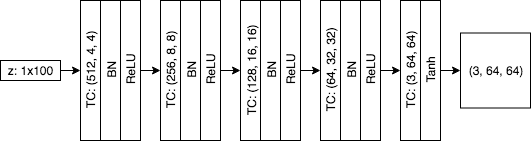
\includegraphics[scale=0.75]{network_structure}
  \caption{\gls{dcgan} \cite{radford:conv_gan} Network Structure}
  \label{fig:network_structure}
\end{figure}

Figure \ref{fig:network_structure} shows the network structure of $G$, with five transposed convolutional (TC)
layers and their output dimensions. Except for the last TC layer, each of the previous four TC layers is
followed by a layer of batch normalization (BN), and a layer of \gls{relu} for activation. The last TC layer
is followed by a Tanh layer for activation. The function of BN and activation layers will be explained later.
The parameters for each layer is detailed in table \ref{table:network_layers}. The network structure is
rather simple, compared with other much larger networks. ResNet, for example, contains a deep cascade of
152 layers.

\begin{table}[h]
  \centering
  \caption{\gls{dcgan} Layer Details}
  \begin{tabular}{l | l | l }
    \toprule
    Layer & Type & Description \\
    \midrule
    1 & TC & $100 \rightarrow 512$ channels, $4 \times 4$ kernel, stride $1$, padding $0$ \\
    2 & BN & $512$ channels\\
    3 & ReLU & $512$ channels \\
    4 & TC & $512 \rightarrow 256$ channels, $4 \times 4$ kernel, stride $2$, padding $1$ \\
    5 & BN & $256$ channels \\
    6 & ReLU & $256$ channels \\
    7 & TC & $256 \rightarrow 128$ channels, $4 \times 4$ kernel, stride $2$, padding $1$ \\
    8 & BN & $128$ channels \\
    9 & ReLU & $128$ channels \\
    10 & TC & $128 \rightarrow 64$ channels, $4 \times 4$ kernel, stride $2$, padding $1$ \\
    11 & BN & $64$ channels \\
    12 & ReLU & $64$ channels \\
    13 & TC & $64 \rightarrow 3$ channels, $4 \times 4$ kernel, stride $2$, padding $1$ \\
    14 & Tanh & 3 channels, final layer \\
    \bottomrule
  \end{tabular}
  \label{table:network_layers}
\end{table}

\section{Transposed Convolutional Layer}

In \gls{cnn}s, convolutional layer extracts various features from the input, essentially performing a
downsampling operation. Transposed convolutional layer \cite{transposed_convolution}, also known as
fractionally strided convolutional layer, or sometime erroneously as deconvolutional layer, on the other
hand performs upsampling on the input.  Upsampling is needed in the generator model to successively map the
$1 \times 100$ random noise input $\boldsymbol{z}$ to a much larger $3 \times 64 \times 64$ output. Upsampling of data is often
done with interpolation, but transposed convolution as a novel approach can map the input to a richer space
than what can be achieved with interpolation. It also offers trainability which makes it useful for neural
networks. Conceptually, if a convolution layer of stride $s$ is run backwards, it can be seen as convolution
layer with stride $1/s$, hence the name fractionally strided convolution.

\subsection{Convolution}

To understand the operation of transposed convolution, it is perhaps natural to start with the regular
convolution first by working through a simple numerical example. With convolution, the input and output
can both have multiple channels. A convolutional kernel has the same number of channels that matches the
the number of input channels. The number of kernels determines the number of output channels, i.e., each
kernel generates one output channel. For instance, for a $2D$ convolution for which the number of input
channels and output channels are both $1$, a single one-channel $2D$ kernel is needed. Let the input be
a $4 \times 4$ matrix $A$:

$$
A =
  \begin{pmatrix}
    1 & 2 & 3 & 4 \\
    4 & 3 & 2 & 1 \\
    1 & 2 & 3 & 4 \\
    4 & 3 & 2 & 1
  \end{pmatrix}
$$

Let the kernel be a $2 \times 2$ matrix $K$:

$$
K =
  \begin{pmatrix}
    1 & 2 \\
    3 & 4
  \end{pmatrix}
$$

In addition to the kernel size $k$ ($2$ in this case),
a convolution can have some extra parameters. Padding size $p$ pads the input with $p$ rows or columns
of zeros at the borders. Stride size $s$ is the step size to slide the kernel. Assume the convolution operates
with $p = 1$ and $s = 2$, that is, $K$ is slid across the zero-padded matrix $B$ with a step of
$2$, from left to right, top to bottom. $B$ is shown below:

$$
B =
  \begin{pmatrix}
    {\color{red}0} & {\color{red}0} & {\color{blue}0} & {\color{blue}0} & 0 & 0 \\
    {\color{red}0} & {\color{red}1} & {\color{blue}2} & {\color{blue}3} & 4 & 0 \\
    0 & 4 & 3 & 2 & 1 & 0 \\
    0 & 1 & 2 & 3 & 4 & 0 \\
    0 & 4 & 3 & 2 & 1 & 0 \\
    0 & 0 & 0 & 0 & 0 & 0
  \end{pmatrix}
$$

When $K$ is slid across $B$, the overlapping entries in $B$ during each step is called a \textit{patch}.
The first two patches are shown in red and blue respectively. At each step, an element-wise inner product
(Frobenius inner product) $\langle K,P \rangle_{F}$ is computed between $K$ and the corresponding patch $P$
and stored as an element in the result matrix $C$:

$$
C =
  \begin{pmatrix}
    4 & 8 & 12 \\
    12 & 25 & 13 \\
    8 & 7 & 1
  \end{pmatrix}
$$

In practice, the sliding-window approach is inefficient for implementation. All practical implementations
use a pair of operations called $im2col$ and $col2im$ to wrap a single matrix multiplication. Since
matrix multiplication is such a fundamental operation that its algorithm has been highly optimized over the
decades, this vindicates the memory overhead caused by $im2col$. To start, flatten $K$ into a row vector
$K_{row}$:

$$
K_{row} =
  \begin{pmatrix}
    1 & 2 & 3 & 4 \\
  \end{pmatrix}
$$

For each patch in $B$ that $K$ convolves with, the entries in that patch are unrolled into a matrix $B_{col}$
made of column vectors:

$$
B_{col} =
  \begin{pmatrix}
    0 & 0 & 0 & 0 & 3 & 1 & 0 & 3 & 1 \\
    0 & 0 & 0 & 4 & 2 & 0 & 4 & 2 & 0 \\
    0 & 2 & 4 & 0 & 2 & 4 & 0 & 0 & 0 \\
    1 & 3 & 0 & 1 & 3 & 0 & 0 & 0 & 0
  \end{pmatrix}
$$

This operation is called $im2col$, namely, image to columns. Now, compute the product $K_{row} * B_{col}$,
a $1 \times 9$ matrix is obtained:

$$
\begin{pmatrix}
  4 & 18 & 12 & 12 & 25 & 13 & 8 & 7 & 1
\end{pmatrix}
$$

Finally this matrix is ``reshaped'' to the desired $3 \times 3$ output $C$ using the operation $col2im$.

\subsection{Represent Convolution as a Sparse Matrix}

The procedure just described in the previous section is how regular convolution would be implemented in
practice. On the other hand, there is an alternative view of the convolution, also performed with a single
matrix multiplication. This alternative view is impractical for implementation, but from which
the input and output can be easily reversed. To see this, first unroll the zero-padded input $B$ into
a $36 \times 1$ matrix:

\setcounter{MaxMatrixCols}{20}

$$
\tilde{B}^\intercal =
  \begin{pmatrix}
    0 & 0 & 0 & 0 & 0 & 0 & 0 & 1 & 2 & 3 & 4 & 0 & 0 & 4 & \dots
  \end{pmatrix}
$$

The output $C$ is also unrolled into a $9 \times 1$ matrix:

$$
\tilde{C}^\intercal =
  \begin{pmatrix}
    4 & 18 & 12 & 12 & 25 & 13 & 8 & 7 & 1
  \end{pmatrix}
$$

Then the convolution can be represented as a sparse matrix $M$ of $9 \times 36$ with entries from kernel $K$,
one patch per row:

$$
M =
  \begin{pmatrix}
    1 & 2 & 0 & 0 & 0 & 0 & 3 & 4 & 0 & 0 & 0 & 0 & \dots \\
    0 & 0 & 1 & 2 & 0 & 0 & 0 & 0 & 3 & 4 & 0 & 0 & \dots \\
    \vdots \\
  \end{pmatrix}
$$

$M$ takes $\tilde{B}$ as input and produces $\tilde{C}$ as output, which again can be reshaped to $C$.

\subsection{Transposed Convolution}

In the previous section, the convolution is represented as a kernel-defined sparse matrix. Under this view,
it is very easy to derive the \textit{backward pass}. The example convolution maps an input of $4 \times 4$
to an output of $3 \times 3$. To reverse the direction of input and output, namely, to take an input of
$3 \times 3$ and produce an output of $4 \times 4$, all it takes is to transpose $M$ to obtain $M^\intercal$
of $36 \times 9$. When $M^\intercal$ is applied to the an $3 \times 3$ input unrolled to $9 \times 1$, the
resulting $36 \times 1$ matrix is then reshaped to the desired $4 \times 4$ output (with a padding of $1$). Hence the name
\textit{transposed convolution}.

It needs to be pointed out that the term \textit{backward pass} instead of \textit{inverse operation} was used,
since $M^\intercal$ does not recover the numerical values of $B$ from $C$, it only recovers the shape of $B$,
therefore it is misleading to call this operation deconvolution. Also, the same kernel $K$ defines both
the forward pass and the backward pass.

The kernel size $k$, padding $p$ and stride $s$ parameters of the convolution affect the corresponding
transposed convolution as well. The detailed relationship is well documented by V. Dumoulin and F. Visin in
\cite{dumoulin:conv_arithmetic}. For instance, the previous convolution example has an input size $i = 4$,
which satisfies the condition $(i + 2p - k \mod s) = 0$, then the associated transposed convolution
(input size $i' = 3$) can be described by a regular convolution on input size $\tilde{i}'$ and parameters
$k' = k$, $s' = 1$ and $p' = k - p - 1$,
where $\tilde{i}'$ is the size when the input is dilated by $s - 1$ zeros between each element. The output
size is

\begin{equation}
  o' = s(i' - 1) + k - 2p.
\end{equation}

Here, $\tilde{i}' = 5$, $k' = 2$, $s' = 1$ and $p' = 0$. The output size $o' = 4$, which equals the
original input size $i$ of the associated convolution. To illustrate this with a numerical example, let
the input $3 \times 3$ matrix be

$$
A' =
  \begin{pmatrix}
    1 & 2 & 3 \\
    3 & 2 & 1 \\
    1 & 2 & 3
  \end{pmatrix}
$$

This matrix needs to be dilated with $s - 1 = 1$ zeros, resulting in

$$
A'' =
  \begin{pmatrix}
    1 & 0 & 2 & 0 & 3 \\
    0 & 0 & 0 & 0 & 0 \\
    3 & 0 & 2 & 0 & 1 \\
    0 & 0 & 0 & 0 & 0 \\
    1 & 0 & 2 & 0 & 3
  \end{pmatrix}
$$

Convolve $A''$ (without padding since $p' = 0$) with the same kernel $K$ using stride $s' = 1$, the result
is

$$
C' =
  \begin{pmatrix}
    1 & 4 & 2 & 6 \\
    9 & 8 & 6 & 4 \\
    3 & 4 & 2 & 2 \\
    3 & 8 & 6 & 12
  \end{pmatrix}
$$

In practice, the transposed convolution can also be implemented with a single matrix multiplication
followed by a $col2im$ operation. The details are explained in chapter 3.

\section{Batch Normalization Layer}

Batch normalization is an operation defined as

\begin{equation} \label{eq:batch_normalization}
  y = \gamma \frac{x - \bar{x}}{\sqrt{\sigma^2(x) + {eps}}} + \beta
\end{equation}

Here $eps$ is a small constant that adds to numerical stability. $\gamma$ and $\beta$ can be regarded
as trained weight and bias. The output $y$ of the normalization would have a mean of $0$ and standard
deviation of $1$. Batch normalization optimizes the training of the network, making it converge
faster with higher learning rates. It can also improve overall accuracy of the model. For deep networks
like \gls{dcgan}, it is a key ingredient.

However, this operation involves an inverse square root operation $\frac{1}{\sqrt{\sigma^2(x) + eps}}$,
which is rather difficult to compute with fixed-point numbers. Luckily Xilinx Vivado includes an IP which
can both convert between fixed-point and floating-point representations, as well as compute the inverse square
root.

\section{Activation Layer}

Activation function, also known as \textit{transfer function}, adds non-linearity to the network. It is often
attached to the output of a layer, typically mapping the results to the range $(0, 1)$ or $(-1, 1)$, albeit
other possibilities exist. Assume the function maps the input to range $(0, 1)$, a value close to $0$ would
be seen as ``off'' or ``no'', a value close to $1$ would be seen as ``on'' or ``yes''. This indicates whether the
following connection should see this output as activated or not, hence the name activation function.

\begin{figure}[h]
  \centering
  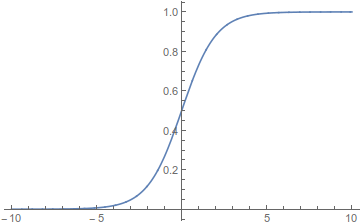
\includegraphics[scale=0.5]{sigmoid}
  \caption{Sigmoid Activation Function}
  \label{fig:sigmoid}
\end{figure}

Many different types of activation functions exist with two main categories: linear and nonlinear. A commonly
used nonlinear sigmoid (S-shaped) function is $y = \frac{1}{1 + e^{-x}}$, shown in figure \ref{fig:sigmoid}.

\subsection{ReLU Layer}

ReLU is very popular nowadays. It is defined as

\begin{equation} \label{eq:relu}
  y = max(0, x)
\end{equation}

\begin{figure}[h]
  \centering
  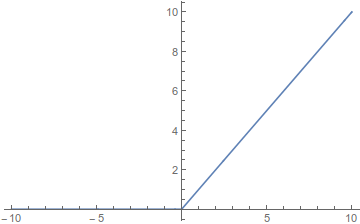
\includegraphics[scale=0.5]{relu}
  \caption{ReLU Activation Function}
  \label{fig:relu}
\end{figure}

As shown in figure \ref{fig:relu}, it is worth noting that ReLU is in fact nonlinear. When compared
with the sigmoid function, the
gradient of ReLU does not saturate when $x$ gets large, which makes \gls{sgd} converge faster. In addition,
since all negative values are converted to zero, it adds the desirable feature of sparsity to the network,
leading to more efficient computation. The implementation of ReLU is of course straightforward.

\subsection{Tanh Layer}

The hyperbolic tangent function $tanh$ is another widely used activation function. It works similarly to the
sigmoid function with the additional property of being symmetrical with respect to the origin. In the \gls{dcgan} model, the Tanh layer is used as the last layer to output the final generated image.

\begin{equation} \label{eq:tanh}
  \begin{split}
    y & = \frac{e^x - e^{-x}}{e^{x} + e^{-x}} \\
      & = \frac{e^{2x} - 1}{e^{2x} + 1} \\
      & = \frac{1- e^{-2x}}{1 - e^{-2x}}
  \end{split}
\end{equation}

\begin{figure}[h]
  \centering
  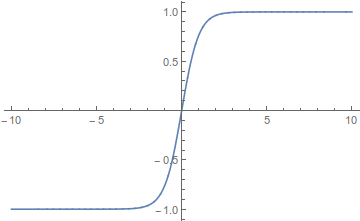
\includegraphics[scale=0.5]{tanh}
  \caption{Tanh Activation Function}
  \label{fig:tanh}
\end{figure}

\clearpage %force the next chapter to start on a new page. Keep that as the last line of your chapter!
